\documentclass[tikz,border=2pt]{standalone}
\usepackage{mathptmx}
\usepackage{amsmath,amssymb}
\usetikzlibrary{arrows.meta,positioning,calc,fit,backgrounds,decorations.pathreplacing}

\definecolor{expert}{HTML}{EB6834}
\definecolor{cand}{HTML}{2A78D6}
\definecolor{critic}{HTML}{1BAF7A}
\definecolor{ink}{HTML}{1F1F1E}
\definecolor{muted}{HTML}{6B6A66}
\definecolor{panel}{HTML}{F6F5F2}
\definecolor{line}{HTML}{B4B2A9}

\tikzset{
  box/.style={draw=line, fill=white, rounded corners=2pt, minimum height=6.5mm, inner xsep=4pt, font=\small, align=center},
  cbox/.style={box, draw=critic, fill=critic!8},
  arr/.style={-{Stealth[length=2.2mm]}, line width=0.6pt, color=ink},
  garr/.style={-{Stealth[length=2.2mm]}, line width=0.6pt, color=critic, dashed},
  ptitle/.style={font=\small\bfseries, anchor=north west, color=ink},
  note/.style={font=\footnotesize, color=muted, align=left},
}

\begin{document}
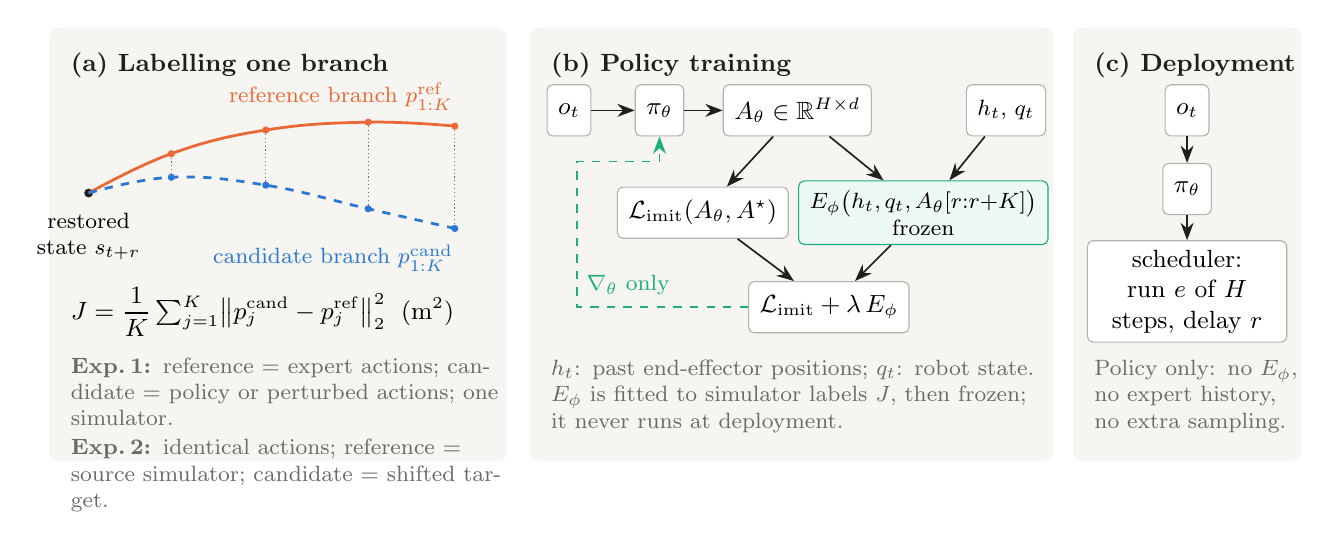
\begin{tikzpicture}

% ------------------------------------------------------------------ panel (a)

  \node[ptitle] at (0, 3.15) {(a) Labelling one branch};
  \fill[ink] (0.35, 1.25) circle (1.6pt);
  \node[font=\footnotesize, anchor=north, align=center] at (0.35, 1.12) {restored\\state $s_{t+r}$};
  % expert branch
  \draw[expert, line width=1pt] plot[smooth, tension=0.7] coordinates {(0.35,1.25) (1.4,1.75) (2.6,2.05) (3.9,2.15) (5.0,2.1)};
  % candidate branch
  \draw[cand, line width=1pt, dashed] plot[smooth, tension=0.7] coordinates {(0.35,1.25) (1.4,1.45) (2.6,1.35) (3.9,1.05) (5.0,0.8)};
  \foreach \x/\ye/\yc in {1.4/1.75/1.45, 2.6/2.05/1.35, 3.9/2.15/1.05, 5.0/2.1/0.8} {
    \draw[muted, line width=0.4pt, densely dotted] (\x,\ye) -- (\x,\yc);
    \fill[expert] (\x,\ye) circle (1.3pt);
    \fill[cand] (\x,\yc) circle (1.3pt);
  }
  \node[font=\footnotesize, color=expert, anchor=south east] at (5.1, 2.18) {reference branch $p^{\mathrm{ref}}_{1:K}$};
  \node[font=\footnotesize, color=cand, anchor=north east] at (5.1, 0.72) {candidate branch $p^{\mathrm{cand}}_{1:K}$};
  \node[font=\small, anchor=north west] at (0.0, 0.18)
     {$J=\dfrac{1}{K}\sum_{j=1}^{K}\bigl\lVert p^{\mathrm{cand}}_{j}-p^{\mathrm{ref}}_{j}\bigr\rVert_2^2$\; (m$^2$)};
  \node[note, anchor=north west, text width=5.5cm] at (0.0, -0.72)
     {\textbf{Exp.\,1:} reference = expert actions; candidate = policy or perturbed actions; one simulator.\\[1pt]
      \textbf{Exp.\,2:} identical actions; reference = source simulator; candidate = shifted target.};

% ------------------------------------------------------------------ panel (b)
\node[ptitle] at (6.1, 3.15) {(b) Policy training};
\node[box] (obs) at (6.45, 2.3) {$o_t$};
\node[box] (pi) at (7.6, 2.3) {$\pi_\theta$};
\node[box] (A) at (9.35, 2.3) {$A_\theta\in\mathbb{R}^{H\times d}$};
\node[box, font=\footnotesize] (hq) at (12.0, 2.3) {$h_t$, $q_t$};
\node[box] (L) at (8.15, 1.0) {$\mathcal{L}_{\mathrm{imit}}(A_\theta, A^\star)$};
\node[cbox, font=\footnotesize] (E) at (10.95, 1.0) {$E_\phi\bigl(h_t, q_t, A_\theta[r{:}r{+}K]\bigr)$\\frozen};
\node[box] (sum) at (9.75, -0.2) {$\mathcal{L}_{\mathrm{imit}}+\lambda\,E_\phi$};
\draw[arr] (obs) -- (pi);
\draw[arr] (pi) -- (A);
\draw[arr] (A) -- (L);
\draw[arr] (A) -- (E);
\draw[arr] (hq) -- (E);
\draw[arr] (L) -- (sum);
\draw[arr] (E) -- (sum);
\draw[garr] (sum.west) -- (6.55,-0.2) -- (6.55,1.65) -| (pi.south);
\node[font=\footnotesize, color=critic, anchor=south west] at (6.55, -0.17) {$\nabla_\theta$ only};
\node[note, anchor=north west, text width=6.2cm] at (6.1, -0.75)
   {$h_t$: past end-effector positions; $q_t$: robot state. $E_\phi$ is fitted to simulator labels $J$, then frozen; it never runs at deployment.};

% ------------------------------------------------------------------ panel (c)
\node[ptitle] at (13.0, 3.15) {(c) Deployment};
\node[box] (o2) at (14.3, 2.3) {$o_t$};
\node[box] (p2) at (14.3, 1.3) {$\pi_\theta$};
\node[box, text width=2.25cm] (s2) at (14.3, 0.0) {scheduler: run $e$ of $H$ steps, delay $r$};
\draw[arr] (o2) -- (p2);
\draw[arr] (p2) -- (s2);
\node[note, anchor=north west, text width=2.6cm] at (13.0, -0.75) {Policy only: no $E_\phi$, no expert history, no extra sampling.};

\begin{scope}[on background layer]
  \fill[panel, rounded corners=3pt] (-0.15,-2.15) rectangle (5.65,3.35);
  \fill[panel, rounded corners=3pt] (5.95,-2.15) rectangle (12.6,3.35);
  \fill[panel, rounded corners=3pt] (12.85,-2.15) rectangle (15.75,3.35);
\end{scope}
\end{tikzpicture}
\end{document}
